%==============================================================================
%  Funnel-Stage SHAP
%
%  Compile:  latexmk -pdf paper.tex        (or pdflatex/bibtex/pdflatex x2)
%
%  Class:    elsarticle (Elsevier). If it is not installed, swap the two lines
%            marked FALLBACK below to use the standard article class; nothing
%            else in this file depends on elsarticle.
%
%  Citations: natbib author-year, giving APA-style (Author, year) with \citep
%            and Author (year) with \citet.
%==============================================================================

\documentclass[review,3p,times,authoryear]{elsarticle}   % <-- FALLBACK: comment out
% \documentclass[11pt,a4paper]{article}                  % <-- FALLBACK: uncomment
% \usepackage[authoryear,round]{natbib}                  % <-- FALLBACK: uncomment

\usepackage[T1]{fontenc}
\usepackage[utf8]{inputenc}
\usepackage{graphicx}
\usepackage{booktabs}
\usepackage{amsmath}
\usepackage{amssymb}
\usepackage{siunitx}
\usepackage{multirow}
\usepackage{array}
\usepackage{caption}
\usepackage{xcolor}
\usepackage[hidelinks]{hyperref}

\graphicspath{{figures/}}
\sisetup{detect-weight=true, detect-family=true}

% Compact helper for a "pass"/"fail" cell against a pre-registered threshold.
\newcommand{\pass}{\textbf{pass}}
\newcommand{\fail}{\textit{fail}}

\journal{Decision Support Systems}

\begin{document}

\begin{frontmatter}

\title{Funnel-Stage SHAP: temporal attribution trajectories and their
       faithfulness in e-commerce purchase prediction}

\author[a]{Ayoub Agnaou}
\affiliation[a]{organization={[Institution]},
                addressline={[Address]},
                city={[City]},
                country={[Country]}}

\begin{abstract}
Conversion prediction from clickstream data is well established, but the
explanations attached to such models are typically computed once over an entire
session and are almost never validated. Both practices are problematic: a
whole-session attribution includes events at or after the purchase decision, and
it cannot express \emph{when} a driver mattered. We propose a funnel-stage SHAP
framework in which Shapley attributions are conditioned on journey stage and
computed strictly on the event prefix available at each stage's cut-point, and we
pair it with an evaluation layer that tests whether the resulting explanations are
faithful, stable and reproducible. The framework is applied to a canonical
session-level benchmark (12,330 sessions) and to an event-level clickstream of
42.4 million events yielding 485,459 sessions. Three results run against
expectation. First, once normalised by its own chance level, predictive
performance \emph{declines} across the funnel (lift 1.79 to 1.09; ROC-AUC 0.641 to
0.569), so conversion becomes harder, not easier, to predict as intent forms.
Second, attribution is strongly non-monotone: navigation entropy carries 3.5\% of
attribution mass at awareness, 22.4\% at consideration and 7.4\% at intent, a
pattern any whole-session analysis averages into a single uninformative value.
Third, cross-paradigm agreement between tree- and recurrent-model attributions
holds at the level of aggregate rankings but disappears at the level of individual
journeys. We argue that explanation quality tracks predictive signal and should
therefore be validated per stage rather than per model.
\end{abstract}

\begin{keyword}
Explainable AI \sep SHAP \sep purchase prediction \sep consumer journey \sep
clickstream analysis \sep design science research
\end{keyword}

\end{frontmatter}

%==============================================================================
\section{Introduction}
%==============================================================================

Online retailers routinely predict whether a browsing session will end in a
purchase, and they act on those predictions: allocating retargeting budget,
triggering on-site interventions, prioritising service contacts. Decisions of that
kind require reasons, not only scores. A model that ranks sessions accurately but
cannot say \emph{why} offers little guidance about what to change
\citep{rudin2019stop}, and the marketing literature has long framed the online
journey as a sequence of qualitatively distinct phases rather than a single
undifferentiated visit \citep{bucklin2003model,lemon2016understanding,moe2003buying}.

Shapley additive explanations \citep{lundberg2017unified}, and their exact and
efficient tree-model variant \citep{lundberg2020local}, have become the default
vehicle for supplying those reasons. In the e-commerce setting they are typically
applied in a particular way: a single model is fitted to session-level aggregates,
and a single attribution is computed per feature over the whole session. We argue
that this common practice carries two defects, one methodological and one
substantive.

\paragraph{The methodological defect is leakage inside the explanation.}
When features are aggregated over an entire session, they necessarily include
events at or after the moment of purchase. The canonical benchmark for this task
illustrates the problem directly: its strongest predictor, \texttt{PageValues}, is
the average value of pages on which a transaction was completed and is therefore
partly a consequence of conversion rather than a cause of it
\citep{sakar2019real}. A model built on such features may predict well and explain
nothing, because the explanation describes the outcome rather than the behaviour
that preceded it.

\paragraph{The substantive defect is temporal flattening.}
A single attribution per feature cannot express that a driver mattered at one
point in the journey and not at another. If the importance of a behavioural signal
genuinely changes as intent forms---which the staged view of the consumer journey
predicts---then a whole-session attribution reports its average, a number that may
correspond to no phase of the journey at all.

\subsection{Positioning relative to existing methods}

Sequence-aware Shapley estimation already exists, and this paper does not propose
a new one. TimeSHAP extends KernelSHAP to recurrent models and produces event-,
timestep- and feature-level attributions \citep{bento2021timeshap}. WindowSHAP
computes Shapley values over time-series windows rather than individual timesteps
\citep{nayebi2023windowshap}. Our contribution is \emph{not} a Shapley estimator.
It is framework-level and domain-level, and consists of three parts:

\begin{enumerate}
  \item \textbf{Funnel-stage conditioning of attributions.} We compute Shapley
        attributions separately at each funnel stage, on the event prefix
        available at that stage, and characterise the resulting
        \emph{attribution trajectory} across stages rather than reporting one
        whole-session attribution.
  \item \textbf{A validation layer for stage-conditioned explanations.} We test
        faithfulness, stability under perturbation, and reproducibility across
        random seeds, with thresholds fixed before any result was computed.
  \item \textbf{Cross-paradigm evidence, tested two ways.} We compare tree-based
        stage attributions against recurrent-model attributions both as aggregate
        rankings and, critically, at the level of individual journeys.
\end{enumerate}

Figure~\ref{fig:gap} positions the work against the three literatures it draws on,
and Figure~\ref{fig:contributions} maps each research question to its
methodological innovation, empirical finding and theoretical contribution.

\begin{figure}[t]
\centering
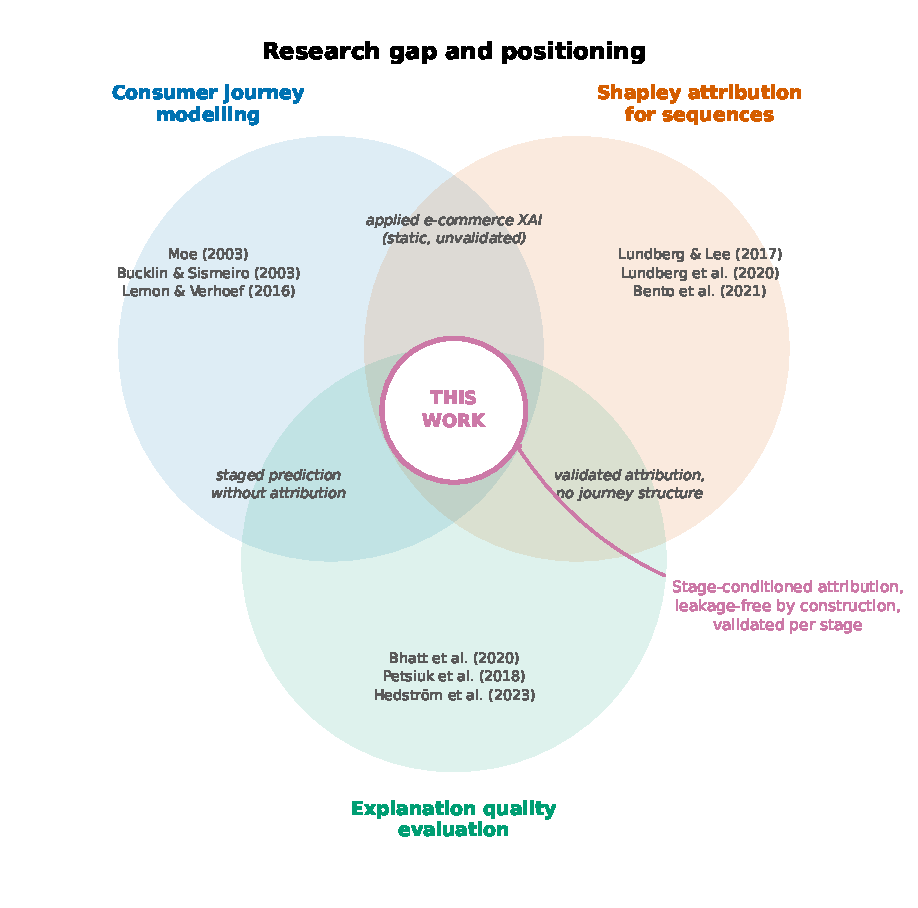
\includegraphics[width=0.86\linewidth]{diag2_gap.pdf}
\caption{Research gap and positioning. Consumer journey modelling supplies the
staged view of the visit; Shapley attribution supplies the estimator; explanation
quality evaluation supplies the validation apparatus. The contribution lies at
their intersection, which is presently sparse in the applied literature.}
\label{fig:gap}
\end{figure}

The study is pre-registered. Every analytic decision was fixed before the test
partition was opened, and each subsequent deviation is recorded with a date and
rationale in a public amendment log (Appendix~A). Twenty-three amendments were
logged, several of which reverse an initial decision on the basis of measurement;
we regard this record as part of the contribution rather than an embarrassment to
be hidden.

\begin{figure*}[t]
\centering
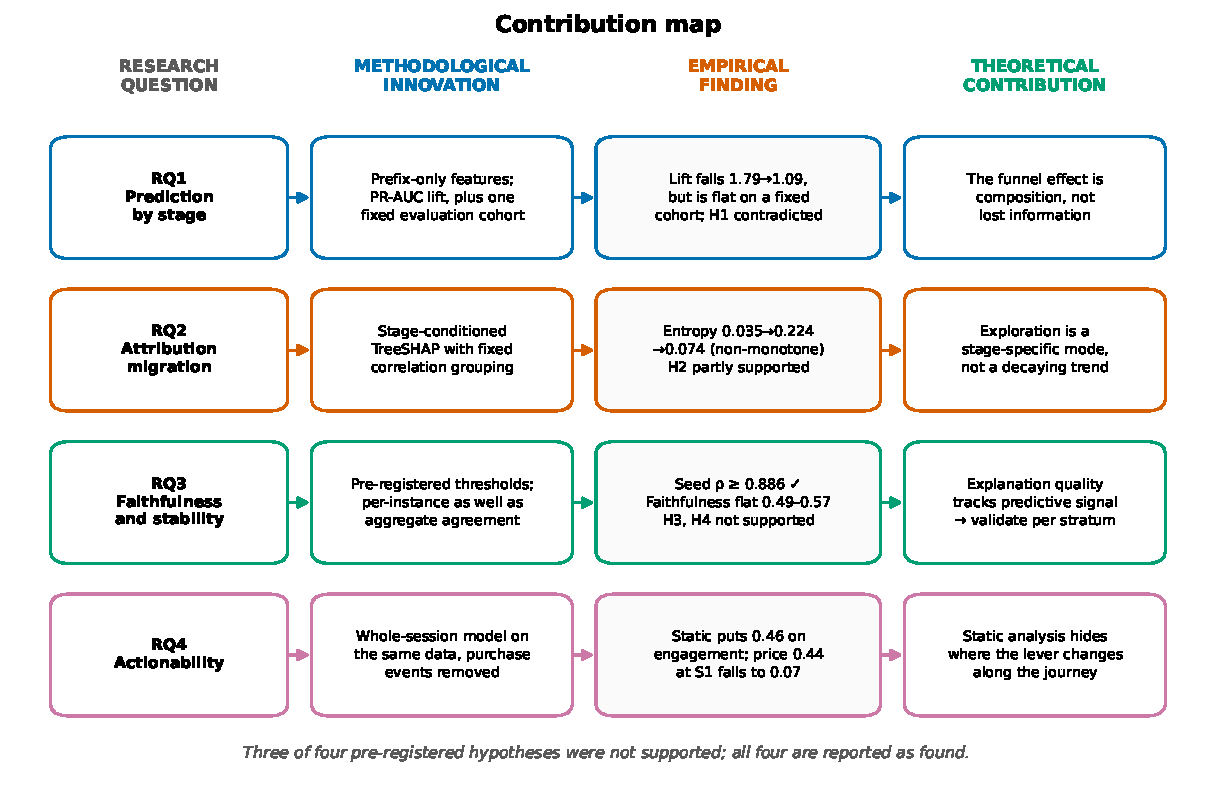
\includegraphics[width=0.94\linewidth]{diag6_contributions.pdf}
\caption{Contribution map. Each research question is traced through its
methodological innovation, the empirical finding it produced, and the theoretical
claim that follows. Three of four pre-registered hypotheses were not supported.}
\label{fig:contributions}
\end{figure*}

%==============================================================================
\section{Related work}
%==============================================================================

\subsection{Purchase prediction from clickstream data}

Modelling online browsing and purchase behaviour has an established tradition in
marketing science, from path analysis of within-site navigation
\citep{montgomery2004modeling} to models of purchase incidence at individual sites
\citep{sismeiro2004modeling,vandenpoel2005predicting}. \citet{moe2003buying} argued
that visits are heterogeneous in purpose---directed buying, search and
deliberation, hedonic browsing, knowledge building---which implies that a single
model of ``the session'' conflates behaviourally distinct processes. The
customer-journey literature makes the same point at a higher level of abstraction,
treating pre-purchase, purchase and post-purchase as separate stages with distinct
drivers \citep{lemon2016understanding}.

The machine-learning literature on the same task has largely proceeded on
session-level aggregates. The UCI Online Shoppers dataset \citep{sakar2019real} is
the canonical benchmark and is dominated by gradient-boosted tree ensembles
\citep{chen2016xgboost,ke2017lightgbm,prokhorenkova2018catboost} and random
forests \citep{breiman2001random}.

\subsection{Shapley attribution for sequential models}

Shapley values provide an additive attribution with desirable axiomatic properties
\citep{lundberg2017unified}, and TreeSHAP makes their computation tractable and
exact for tree ensembles \citep{lundberg2020local}. Two caveats matter here.
First, attributions computed under the path-dependent estimator can assign credit
to features merely correlated with those the model uses; the interventional
estimator, computed against an explicit background distribution, weakens that
dependence \citep{lundberg2020local}. Second, Shapley values are unreliable under
strong feature dependence more generally \citep{aas2021explaining}, which motivates
grouping correlated features before ranking them.

For sequential data, TimeSHAP \citep{bento2021timeshap} adapts KernelSHAP to
recurrent models, adding temporal-coalition pruning to keep computation tractable
and producing attributions at event, timestep and feature level. WindowSHAP
\citep{nayebi2023windowshap} attributes to time windows. Both address \emph{how to
compute} Shapley values on sequences. Neither addresses which \emph{decision point}
the attribution should be conditioned on, which is the question this paper takes up.

\subsection{Evaluating explanations}

That an explanation is produced does not make it faithful to the model.
\citet{bhatt2020evaluating} formalise faithfulness as the correlation between the
attribution assigned to a feature subset and the change in prediction when that
subset is removed. Deletion and insertion curves offer a complementary view,
measuring how quickly a prediction degrades as highly-attributed features are
removed \citep{petsiuk2018rise}. Stability is typically operationalised as a
local-Lipschitz bound on attribution change under small input perturbation
\citep{alvarezmelis2018robustness}, and toolkits now exist to standardise such
measurements \citep{hedstrom2023quantus}. Explanations are also known to be
manipulable and therefore worth verifying rather than trusting
\citep{slack2020fooling}.

\textcolor{red}{\textbf{[UNVERIFIED CLAIM --- resolve before submission.]}} Our
impression is that applied e-commerce XAI studies rarely apply any of these tests,
reporting SHAP summary plots without validation. This claim requires a systematic
review before it can be stated as written; it currently rests on informal reading
and is the single most load-bearing gap-claim in the paper.

\subsection{Positioning}

Table~\ref{tab:positioning} places this work against the methods above.

\begin{table*}[t]
\centering
\caption{Positioning against existing Shapley and explanation-evaluation methods.}
\label{tab:positioning}
\small
\begin{tabular}{@{}p{3.1cm}p{2.6cm}p{2.4cm}p{3.4cm}p{2.2cm}@{}}
\toprule
\textbf{Work} & \textbf{Attribution grain} & \textbf{Decision point} &
\textbf{Validated?} & \textbf{Domain} \\
\midrule
\citet{lundberg2017unified} & feature, per instance & n/a & axioms only & general \\
\citet{lundberg2020local}   & feature, per instance & n/a & axioms only & general (trees) \\
\citet{bento2021timeshap}   & event / timestep / feature & whole sequence & partial & general (recurrent) \\
\citet{nayebi2023windowshap}& time window & whole sequence & partial & time series \\
Typical applied e-commerce XAI & feature, whole session & whole session & rarely & e-commerce \\
\textbf{This work} & \textbf{feature, per funnel stage} &
\textbf{stage cut-point (prefix only)} &
\textbf{faithfulness, stability, seed and cross-paradigm consistency} &
\textbf{e-commerce} \\
\bottomrule
\end{tabular}
\end{table*}

%==============================================================================
\section{Materials and methods}
%==============================================================================

\subsection{Research design}

The study follows a design-science frame \citep{hevner2004design}: the artefact is
the funnel-stage SHAP framework, and each (model $\times$ stage $\times$
explanation) combination constitutes a build--evaluate cycle assessed on
predictive utility, explanation quality and statistical rigour.
Figure~\ref{fig:dsr} maps the artefact, its evaluation and the resulting knowledge
contribution onto that frame; Figure~\ref{fig:architecture} gives the
corresponding computational pipeline.

\begin{figure*}[t]
\centering
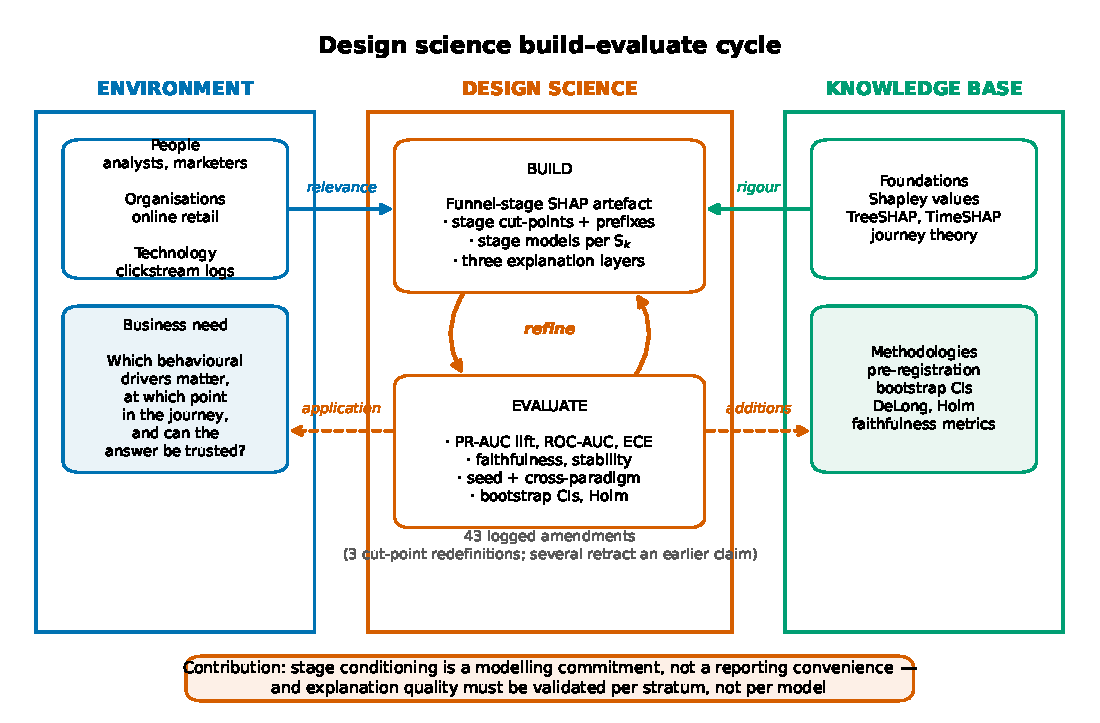
\includegraphics[width=0.92\linewidth]{diag4_dsr.pdf}
\caption{Design science build--evaluate cycle. The relevance cycle draws the
business need from the environment; the rigour cycle draws methods from the
knowledge base; the internal cycle iterates between building the artefact and
evaluating it. The 23 logged amendments are the visible trace of that iteration.}
\label{fig:dsr}
\end{figure*}

\begin{figure*}[t]
\centering
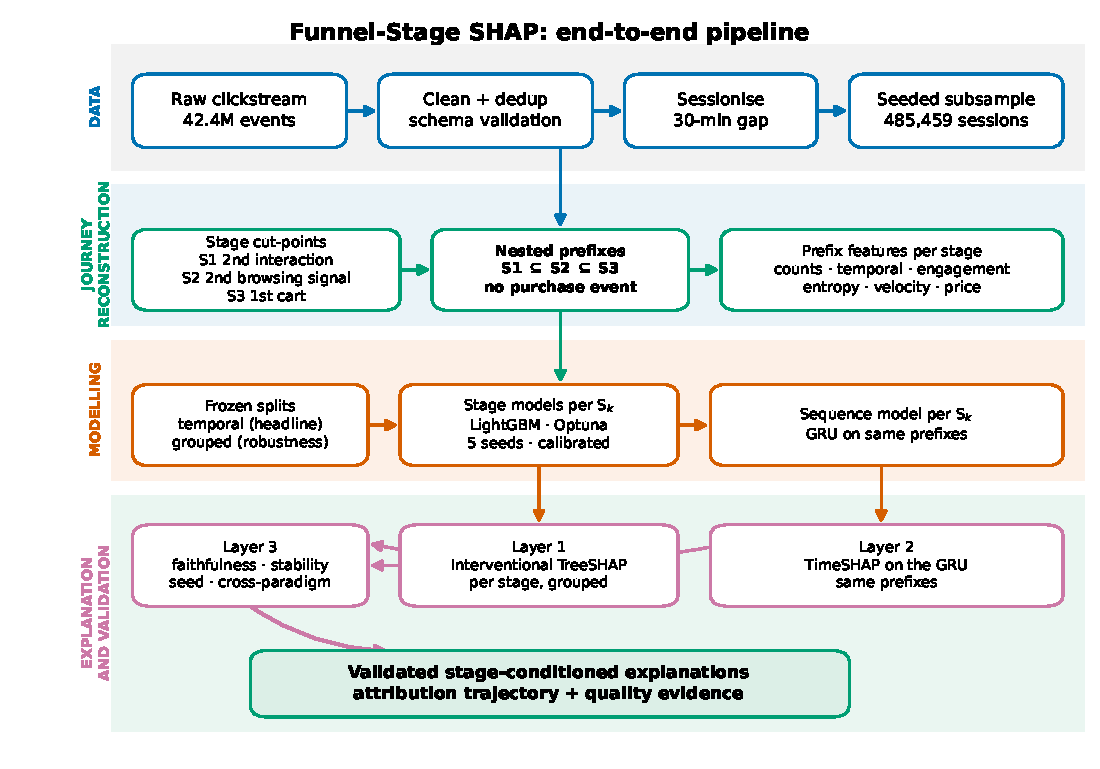
\includegraphics[width=0.94\linewidth]{diag1_architecture.pdf}
\caption{End-to-end pipeline, from raw clickstream to validated
stage-conditioned explanations. Layers~1 and~2 are parallel attribution sources
over the same prefixes; Layer~3 validates both.}
\label{fig:architecture}
\end{figure*}

The analysis is pre-registered. All analytic decisions---stage definitions,
feature families, model families, metrics, statistical tests and pass
thresholds---were fixed in a protocol document before the test partition was
opened. The test partition was read once, at final evaluation. Deviations after
freeze are logged with date, rationale and affected sections (Appendix~A).

\subsection{Data}

Two datasets are used, at deliberately different grains.

\textbf{Dataset A} is the UCI Online Shoppers Purchasing Intention dataset
\citep{sakar2019real}: 12,330 sessions described by 10 numeric and 7 categorical
session-level aggregates, with a binary \texttt{Revenue} target at 15.47\%
prevalence. It serves as a reproducible benchmark and as the static counterpart
against which stage-conditioning is contrasted. Because its features are
whole-session aggregates, models fitted to it are flagged \textbf{non-causal}
throughout.

\textbf{Dataset B} is an event-level clickstream published by the REES46 Marketing
Platform, covering a multi-category online store. We use October 2019: 42,448,764
raw events with fields \texttt{event\_time}, \texttt{event\_type} $\in$
\{view, cart, remove\_from\_cart, purchase\}, \texttt{product\_id},
\texttt{category\_id}, \texttt{brand}, \texttt{price}, \texttt{user\_id} and
\texttt{user\_session}. After cleaning and sessionisation this yields 485,459
sessions from a seeded sample of 200,000 users.

Table~\ref{tab:availability} reports variable availability honestly. Of ten
idealised journey variables, two are absent from both datasets. Search-query text
does not appear in either. Scroll depth is proxied by product-page dwell time and
is never described as scroll depth in results. Device and traffic source are
present in Dataset~A and absent from Dataset~B, which constrains the hypotheses
testable on each.

\begin{table}[t]
\centering
\caption{Availability of the ten idealised journey variables. Two are absent from
both datasets and are reported as limitations rather than proxied silently.}
\label{tab:availability}
\small
\begin{tabular}{@{}lllp{5.1cm}@{}}
\toprule
\textbf{Variable} & \textbf{Dataset A} & \textbf{Dataset B} & \textbf{Note} \\
\midrule
Page views      & present & present & A: page-type counts; B: view events \\
Session duration& present & present & B: last minus first event time \\
Device          & present & \textbf{absent} & B has no device field \\
Traffic source  & present & \textbf{absent} & Constrains H2 on Dataset~B \\
Time of day     & proxy   & present & A: month and weekend only \\
Bounce          & present & proxy   & B: single-event sessions \\
Cart events     & \textbf{absent} & present & Core to stage S3 \\
Search queries  & \textbf{absent} & \textbf{absent} & Limitation; no proxy claimed \\
Scroll depth    & proxy   & proxy   & Product-page dwell time \\
Purchase        & present & present & The label \\
\bottomrule
\end{tabular}
\end{table}

\subsection{Cleaning, sessionisation and subsampling}

Events with null values in \texttt{user\_session}, \texttt{event\_time} or
\texttt{event\_type}, unparseable timestamps, or event types outside the expected
vocabulary were removed, as were exact duplicates on (\texttt{user\_id},
\texttt{event\_time}, \texttt{event\_type}, \texttt{product\_id}). Sessions were
derived by cutting each user's time-ordered event stream on a 30-minute inactivity
gap. We treat the 30-minute rule as a \emph{choice} rather than a standard and
report a 15/30/60-minute sensitivity analysis in Section~\ref{sec:sensitivity}.
Sessions of fewer than two events were dropped, as were sessions above the 99.5th
percentile of length or duration. Figure~\ref{fig:flow} presents the resulting data
flow.

\begin{figure}[t]
\centering
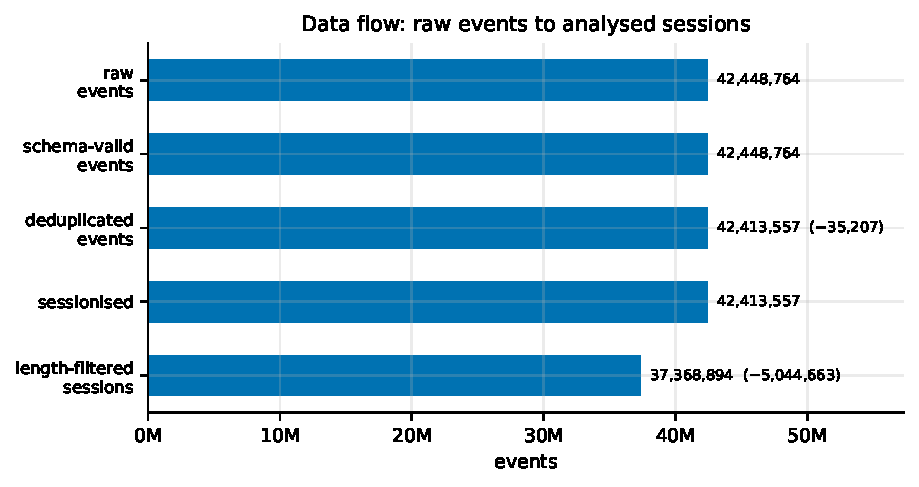
\includegraphics[width=\linewidth]{fig1_data_flow.pdf}
\caption{Data flow from raw events to analysed sessions. Each bar reports the
surviving event count and, in parentheses, the number removed by that filter.}
\label{fig:flow}
\end{figure}

For tractability the analysis uses a seeded random sample of 200,000 users,
retaining every session belonging to a sampled user. Sampling is by \emph{user},
not by session, because both splitting protocols keep visitors whole; sampling
sessions independently would fragment users before the splitter saw them. The
sample is a deterministic hash of (seed, user id), so it is stable across reruns
and nested across sample sizes---a property used in the sample-size sensitivity
analysis.

\subsection{Funnel stages and the anti-leakage prefix protocol}
\label{sec:stages}

This is the scientific core of the design. Four stages are defined on the event
sequence, each with an explicit cut-point, and \textbf{features at stage $S_k$ are
computed only on the event prefix up to that cut-point}. The prefixes therefore
nest, $S_1 \subseteq S_2 \subseteq S_3$, and no prefix may contain a purchase event.

Three cut-point definitions were amended during development, each on the basis of
measurement. We report the amendments because the reasoning is instructive and
because a definition that merely happens to work invites less confidence than one
that was corrected.

\begin{itemize}
  \item \textbf{S1 (awareness)} closes at the \emph{second} product interaction.
        The original definition---the first view---produced a single-event prefix
        in which 19 of 23 features were constant, which would have made any
        improvement curve an artefact of S1 having no features.
  \item \textbf{S2 (consideration)} opens on the \emph{second} browsing signal (a
        repeat product view or a category switch on a view event). Requiring only
        the first signal placed S2's cut-point on the same event as S1's for
        82.8\% of sessions.
  \item \textbf{S3 (intent)} opens at the first cart event. A stage whose trigger
        fires out of funnel order is treated as \emph{unreached} rather than
        advanced to a later position; the alternative made 45.1\% of S2 and S3
        prefixes identical on real data.
  \item \textbf{S4 (conversion)} is defined for descriptive purposes only. Its
        cut-point is the purchase event, which is the label, so no S4 feature
        matrix can exist without leakage.
\end{itemize}

Figure~\ref{fig:prefix} works the protocol through a single session, with
categories shown so that each cut-point can be verified against the stated rule
rather than taken on trust. Table~\ref{tab:stages} reports the resulting stage
populations.

\begin{figure*}[t]
\centering
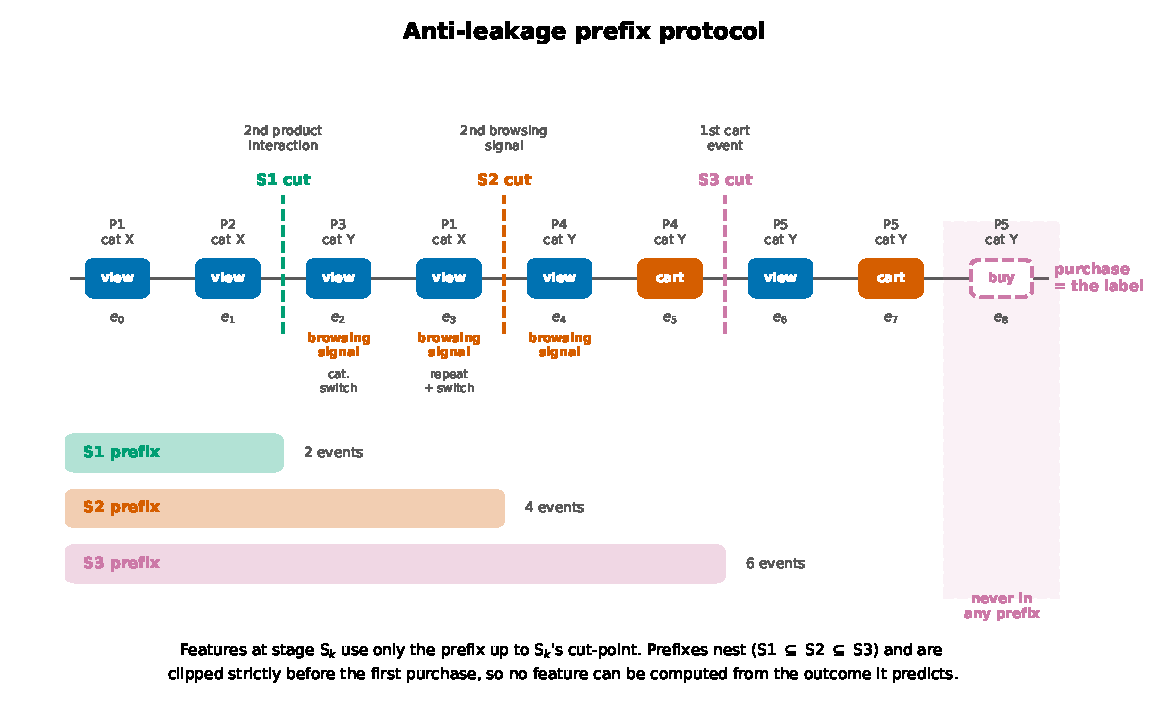
\includegraphics[width=0.96\linewidth]{diag3_prefix.pdf}
\caption{Anti-leakage prefix protocol on a worked session. Browsing signals are
marked so the S2 cut-point (the \emph{second} such signal) is auditable: $e_2$ is
a category switch, $e_3$ is both a repeat view and a switch. Prefixes nest and
are clipped strictly before the purchase.}
\label{fig:prefix}
\end{figure*}

\begin{table}[t]
\centering
\caption{Funnel stages, cut-points and resulting populations on Dataset~B
(200,000-user sample, 30-minute sessionisation gap).}
\label{tab:stages}
\small
\begin{tabular}{@{}llS[table-format=6.0]S[table-format=2.1]S[table-format=2.2]@{}}
\toprule
\textbf{Stage} & \textbf{Cut-point} & {\textbf{N}} & {\textbf{Reach (\%)}} &
{\textbf{Prevalence (\%)}} \\
\midrule
S1 & 2nd product interaction & 475140 & 97.9 & 8.85 \\
S2 & 2nd browsing signal     & 233160 & 48.0 & 6.83 \\
S3 & 1st cart event          & 45031  & 9.3  & 52.10 \\
S4 & purchase / session end  & 485459 & 100.0 & 10.78 \\
\bottomrule
\end{tabular}
\end{table}

Two consequences of this design must travel with every result derived from it.
First, the stage models are \textbf{conditional on reaching the stage}: a session
with no cart has no S3 prefix. Second, prevalence differs sharply by stage, which
makes raw PR-AUC incomparable across stages.

\subsection{Feature engineering}

Features are grouped into families: behavioural counts, temporal features,
engagement, navigation entropy, click velocity, category transitions, a
purchase-intent composite with documented (not fitted) weights, and price context.
Navigation entropy is the Shannon entropy of the category distribution within the
prefix, capturing focus versus wandering.

Two definitional details are load-bearing. \textbf{Dwell time} on an event is the
interval to the following event, and is defined only when that following event
lies inside the same prefix; the final event of a prefix contributes no dwell,
since computing it would require an event past the cut-point.
\textbf{Cart-count features are excluded entirely}: because S3's cut-point is the
\emph{first} cart event, its prefix contains exactly one cart event by
construction, so cart count, removal count and cart recency are constants on every
dataset.

\subsection{Splitting}

Two protocols are used. The \textbf{temporal split} (headline) assigns each user to
a period by their first session and cuts on that boundary, so it is simultaneously
ordered in time and identity-clean. This is stricter than the protocol required: a
purely date-based cut would still allow a returning visitor to appear on both sides.
Users whose activity straddles a boundary are dropped and counted rather than
reassigned. The \textbf{grouped split} (robustness) partitions by user at random. A
naive random split by session is never used.

For Dataset~A neither protocol applies---there is no user identifier, and the only
temporal field is a month name---so sessions are partitioned on month boundaries
chosen by exhaustive search for the split closest to 70/15/15.

\subsection{Explanation protocol}

\paragraph{Layer 1 --- stage-conditioned TreeSHAP.}
Interventional TreeSHAP \citep{lundberg2020local} is computed per stage against a
background sample drawn from training rows only. Correlated features are clustered
by absolute Spearman correlation and their attributions summed, since Shapley
values are additive \citep{aas2021explaining}. The clustering is fixed across
stages and taken from the earliest stage, which is the coarsest: at S1 a two-event
prefix renders seven engagement and temporal features numerically identical, so
their individual attributions there are arbitrary partitions of a single quantity.
Attributions are computed on the validation partition, not the test partition,
which is reserved for predictive evaluation.

\paragraph{Layer 2 --- recurrent attribution.}
A GRU is trained per stage on the \emph{same prefixes} as the tree models and
explained with TimeSHAP \citep{bento2021timeshap}. Training the recurrent model on
whole sessions would have let it see the purchase event, breaking the prefix
protocol for that arm alone and rendering any comparison meaningless.

\paragraph{Layer 3 --- explanation quality.}
Faithfulness is measured by the \citet{bhatt2020evaluating} correlation and by
deletion and insertion curves \citep{petsiuk2018rise}, with removal implemented as
replacement by a background value rather than by zero---zero is a valid
in-distribution value for most of these features and does not remove information.
Deletion orders features by \emph{signed} attribution, since the claim being tested
is that removing features which push the prediction up causes it to fall. Stability
is a local-Lipschitz estimate \citep{alvarezmelis2018robustness}. Consistency is
Spearman rank correlation of importance orderings across the five seeds and between
the two paradigms. Pass thresholds were fixed in advance: faithfulness correlation
$>0.5$, cross-paradigm Spearman $>0.6$. Figure~\ref{fig:validation} summarises the
workflow together with the verdicts it produced.

\begin{figure*}[t]
\centering
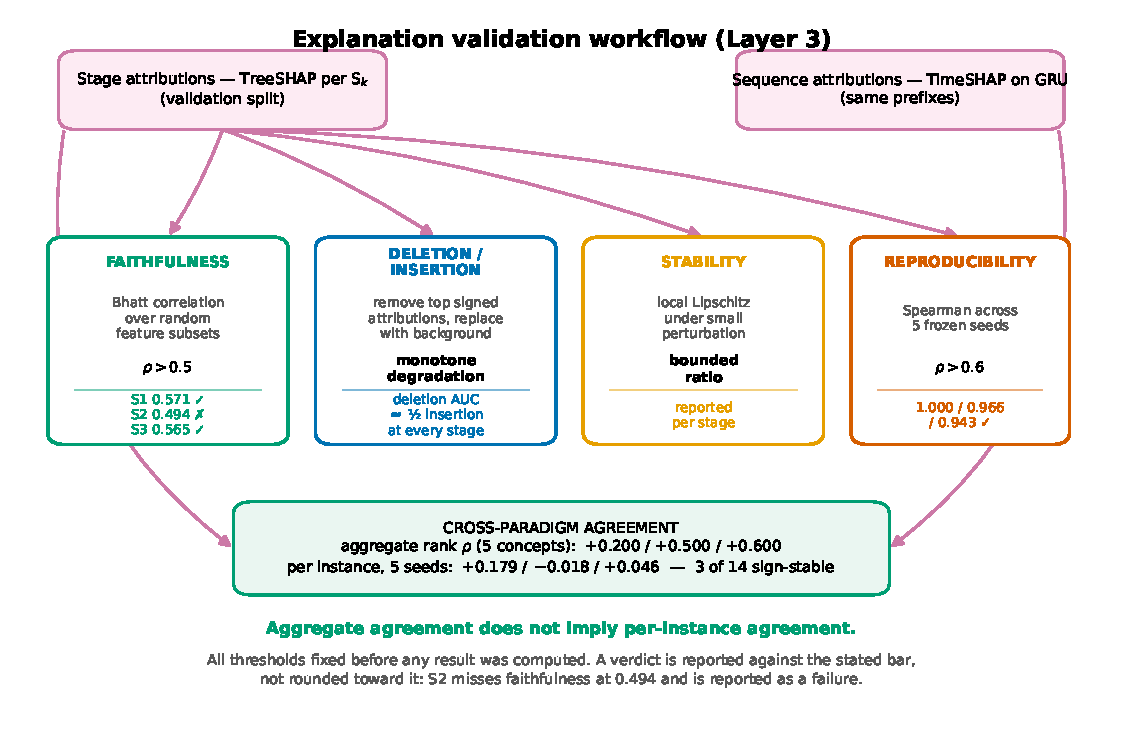
\includegraphics[width=0.94\linewidth]{diag5_validation.pdf}
\caption{Explanation validation workflow. Four tests operate on the tabular
attributions; cross-paradigm agreement requires both sources. Thresholds were
fixed before any result was computed, and each verdict is reported against the
stated bar rather than rounded toward it.}
\label{fig:validation}
\end{figure*}

\subsection{Modelling and evaluation}
\label{sec:eval}

Five model families were evaluated on Dataset~A---logistic regression, random
forest \citep{breiman2001random}, XGBoost \citep{chen2016xgboost}, LightGBM
\citep{ke2017lightgbm} and CatBoost \citep{prokhorenkova2018catboost}---and LightGBM
was carried forward to the stage models. Hyperparameters were tuned with Optuna
\citep{akiba2019optuna} over fixed search spaces, using a held-out validation set
rather than nested cross-validation, because the temporal split forbids shuffling
folds across the time boundary. Class imbalance was handled by class weighting
inside training folds only; SMOTE \citep{chawla2002smote} was available but not used
in the reported runs.

\textbf{PR-AUC is the primary metric}, as appropriate under class imbalance
\citep{davis2006relationship,saito2015precision}. Because chance-level PR-AUC equals
the prevalence, and prevalence differs by a factor of six across stages
(Table~\ref{tab:stages}), we report \textbf{PR-AUC lift}---PR-AUC divided by
prevalence---as the cross-stage comparison, alongside the prevalence-free ROC-AUC.
Reporting raw PR-AUC across stages would report prevalence as though it were skill.

Probability calibration follows \citet{niculescu2005predicting}, fitted isotonically
on a dedicated calibration split carved from the \emph{training} period. Calibration
quality is reported as Brier score and Expected Calibration Error
\citep{guo2017calibration}. Every metric is reported as a mean over five frozen
seeds; between-model differences carry paired bootstrap confidence intervals over
2,000 stratified resamples. Paired ROC-AUC comparisons use the DeLong test
\citep{delong1988comparing} in the fast formulation of \citet{sun2014fast}, vendored
and unit-tested against a naive transcription of the original definition. Multiple
comparisons are corrected by the Holm procedure \citep{holm1979simple} across the
entire pre-declared family; \citet{benjamini1995controlling} is available as an
alternative.

%==============================================================================
\section{Results}
%==============================================================================

\subsection{Data flow and descriptive statistics}

Cleaning and sessionisation reduced 42,448,764 raw events to 37,368,894 events in
5,366,181 sessions, from which the seeded 200,000-user sample retains 485,459
sessions (Figure~\ref{fig:flow}). Stage populations and prevalences are given in
Table~\ref{tab:stages}.

The stage structure itself carries a finding. Conversion prevalence is \textbf{not
monotone} across the funnel: 8.85\% at S1, 6.83\% at S2, 52.10\% at S3.
Consideration selects \emph{against} conversion, because visitors who cart early
are, by the ordering rule, recorded as skipping consideration, and those visitors
convert at much higher rates.

\subsection{Predictive performance (RQ1, H1)}

Dataset~A results are reported in Table~\ref{tab:baselines}, on the month-ordered
split with December held out, over five seeds. Logistic regression's zero standard
deviation is correct rather than anomalous: with a fixed split and a convex
objective the fit is deterministic.

\begin{table}[t]
\centering
\caption{Dataset~A baselines, month-ordered split, test = December, five seeds.
ECE is Expected Calibration Error before and after isotonic calibration on a
training-period slice.}
\label{tab:baselines}
\small
\begin{tabular}{@{}lS[table-format=1.4]@{\,$\pm$\,}S[table-format=1.4]S[table-format=1.4]S[table-format=1.4]S[table-format=1.4]@{}}
\toprule
\textbf{Model} & \multicolumn{2}{c}{\textbf{PR-AUC}} & {\textbf{ROC-AUC}} &
{\textbf{ECE (uncal.)}} & {\textbf{ECE (cal.)}} \\
\midrule
CatBoost            & 0.6994 & 0.0060 & 0.9045 & 0.0629 & 0.0184 \\
Random forest       & 0.6852 & 0.0060 & 0.9071 & 0.0963 & 0.0154 \\
LightGBM            & 0.6770 & 0.0075 & 0.8930 & 0.0654 & 0.0260 \\
XGBoost             & 0.6764 & 0.0045 & 0.8971 & 0.0363 & 0.0179 \\
Logistic regression & 0.5828 & 0.0000 & 0.8768 & 0.2032 & 0.0322 \\
\bottomrule
\end{tabular}
\end{table}

Dataset~B stage models are reported in Table~\ref{tab:stagemodels} and
Figure~\ref{fig:curve}.

\begin{table}[t]
\centering
\caption{Dataset~B stage models (LightGBM, five seeds, temporal split). PR-AUC lift
is PR-AUC divided by prevalence, i.e.\ performance relative to the stage's own
chance level.}
\label{tab:stagemodels}
\small
\begin{tabular}{@{}lS[table-format=5.0]S[table-format=1.3]S[table-format=1.4]@{\,$\pm$\,}S[table-format=1.4]S[table-format=1.2]S[table-format=1.4]S[table-format=1.3]@{}}
\toprule
\textbf{Stage} & {\textbf{N (test)}} & {\textbf{Prev.}} &
\multicolumn{2}{c}{\textbf{PR-AUC}} & {\textbf{Lift}} & {\textbf{ROC-AUC}} &
{\textbf{ECE}} \\
\midrule
S1 & 38059 & 0.073 & 0.1312 & 0.0009 & 1.79 & 0.6406 & 0.010 \\
S2 & 17884 & 0.059 & 0.0834 & 0.0015 & 1.41 & 0.6198 & 0.011 \\
S3 & 2973  & 0.521 & 0.5681 & 0.0041 & 1.09 & 0.5695 & 0.017 \\
\bottomrule
\end{tabular}
\end{table}

\begin{figure}[t]
\centering
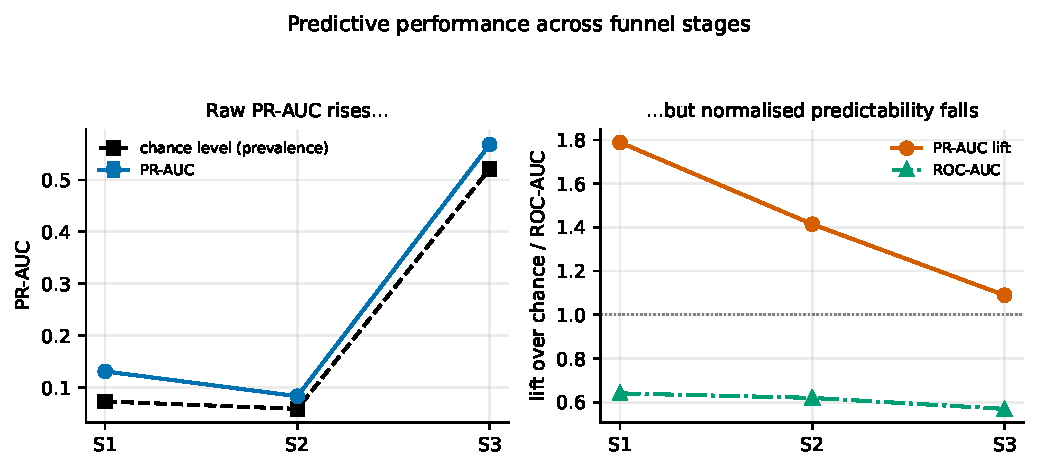
\includegraphics[width=\linewidth]{fig2_improvement_curve.pdf}
\caption{Predictive performance across funnel stages. Left: raw PR-AUC rises, but
so does the chance level (prevalence), which it tracks closely. Right: normalised
by chance, predictability falls monotonically; ROC-AUC, which is
prevalence-independent, falls with it.}
\label{fig:curve}
\end{figure}

\textbf{H1 is not supported; the direction of the effect is reversed.} H1 predicted
that PR-AUC would rise monotonically from awareness to intent. Raw PR-AUC does
rise, from 0.131 to 0.568---but chance-level PR-AUC rises with it, from 0.073 to
0.521. Normalised, the curve runs the other way: lift falls monotonically from 1.79
to 1.09, and ROC-AUC, which is prevalence-independent and therefore cannot be
explained by base rates, falls with it from 0.641 to 0.569. Seed standard
deviations of 0.0009--0.0041 are one to two orders of magnitude smaller than the
between-stage differences. By the intent stage the model is barely above its own
base rate.

\subsection{Feature-family ablation (H3)}

Table~\ref{tab:ablation} reports the ablation, with paired bootstrap 95\%
confidence intervals over the Holm-corrected family of nine contrasts declared in
Section~\ref{sec:eval}.

\begin{table*}[t]
\centering
\caption{Ablation contrasts with paired bootstrap 95\% confidence intervals
(2,000 stratified resamples, Holm-corrected across the nine-contrast family).
Intervals excluding zero are shown in bold.}
\label{tab:ablation}
\small
\begin{tabular}{@{}lccc@{}}
\toprule
\textbf{Stage} & \textbf{+temporal vs baseline} &
\textbf{entropy/velocity vs baseline (H3)} &
\textbf{entropy/velocity given temporal} \\
\midrule
S1 & \textbf{+0.0102} [+0.0045, +0.0167] & +0.0038 [$-$0.0002, +0.0084] & $-$0.0006 [$-$0.0017, +0.0005] \\
S2 & \textbf{+0.0120} [+0.0057, +0.0197] & +0.0035 [$-$0.0011, +0.0085] & +0.0007 [$-$0.0017, +0.0031] \\
S3 & +0.0139 [$-$0.0074, +0.0370]        & +0.0156 [$-$0.0027, +0.0346] & +0.0018 [$-$0.0045, +0.0085] \\
\bottomrule
\end{tabular}
\end{table*}

\textbf{H3 is not supported.} The interval for entropy and click-velocity features
against baseline aggregates covers zero at every stage. The temporal family, by
contrast, contributes reliably at S1 and S2.

The robust result here is the \textbf{redundancy}: given the temporal family,
entropy and velocity add nothing, and those are the only intervals narrow enough to
distinguish ``no effect'' from ``cannot tell''. This is mechanically unsurprising---
click velocity is events divided by elapsed prefix duration, so both of its
constituents are temporal features.

No S3 contrast is decidable. With 2,973 test sessions every intent-stage interval
spans roughly $\pm 0.02$, admitting both a meaningful gain and a meaningful loss.
This is a power limitation, not a null result.

\subsection{Attribution migration (RQ2, H2)}

Figure~\ref{fig:migration} presents the attribution trajectories;
Table~\ref{tab:migration} gives the underlying shares of total mean $|$SHAP$|$ by
correlation group.

\begin{figure}[t]
\centering
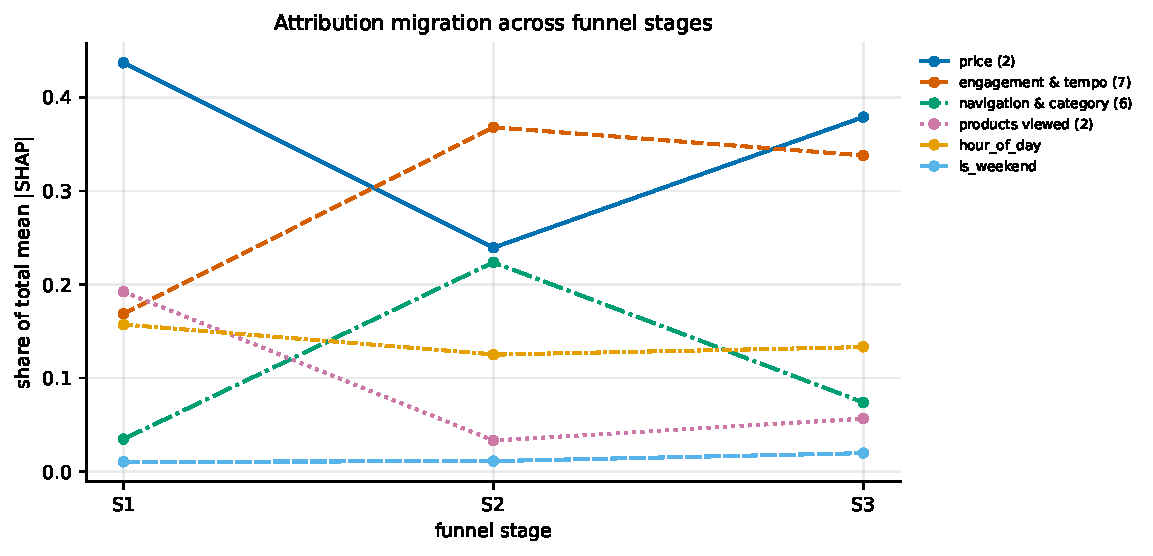
\includegraphics[width=\linewidth]{fig3_attribution_migration.pdf}
\caption{Attribution migration across funnel stages. Shares of total mean
$|$SHAP$|$ per correlation group; groups are fixed across stages and derived from
the earliest (coarsest) stage. Within a merged group, later-stage migration is not
visible.}
\label{fig:migration}
\end{figure}

\begin{table}[t]
\centering
\caption{Share of total mean $|$SHAP$|$ by driver group and funnel stage
(interventional TreeSHAP, background 500, 2{,}000 validation sessions per stage).}
\label{tab:migration}
\small
\begin{tabular}{@{}lS[table-format=1.3]S[table-format=1.3]S[table-format=1.3]S[table-format=+1.3]@{}}
\toprule
\textbf{Driver group} & {\textbf{S1}} & {\textbf{S2}} & {\textbf{S3}} &
{\textbf{$\Delta$ (S1$\to$S3)}} \\
\midrule
Price (2 features)          & 0.437 & 0.239 & 0.379 & -0.058 \\
Engagement and tempo (7)    & 0.169 & 0.368 & 0.338 & +0.169 \\
Products viewed (2)         & 0.192 & 0.033 & 0.057 & -0.136 \\
Navigation and category (6) & 0.035 & 0.224 & 0.074 & +0.039 \\
Hour of day                 & 0.157 & 0.125 & 0.133 & -0.024 \\
Weekend                     & 0.010 & 0.011 & 0.020 & +0.009 \\
\bottomrule
\end{tabular}
\end{table}

Both stage pairs are fully distinct---no session shares a cut-point between S1 and
S2 or between S2 and S3 (mean gaps 2.49 and 5.37 events)---so the trajectories
compare genuinely different prefixes.

\textbf{H2 is partially supported.} Its behavioural arm holds: attribution to
engagement and tempo doubles from 0.169 at awareness to 0.338 at intent, the largest
single shift in the table. Its context arm \textbf{cannot be tested on Dataset~B},
because traffic source and device are absent from the schema
(Table~\ref{tab:availability}). Price leads at S1 and is the nearest available
product-context proxy, but it is a product attribute rather than an acquisition
channel and we do not present it as one.

The more interesting result is one H2 did not anticipate. \textbf{Navigation
entropy is strongly non-monotone}, rising from 3.5\% of attribution mass at
awareness to 22.4\% at consideration before falling to 7.4\% at intent. Exploratory
breadth is a \emph{stage-specific} signal: it matters where the visitor is choosing
among alternatives and ceases to matter once they have chosen.

\subsection{Explanation quality (RQ3)}

Table~\ref{tab:quality} and Figure~\ref{fig:quality} report Layer~3.

\begin{table*}[t]
\centering
\caption{Explanation quality by stage. Thresholds (faithfulness $>0.5$, seed
Spearman $>0.6$) were fixed before any result was computed.}
\label{tab:quality}
\small
\begin{tabular}{@{}lcccccc@{}}
\toprule
\textbf{Stage} & \textbf{Faithfulness $\rho$} & \textbf{vs 0.5} &
\textbf{Deletion AUC} & \textbf{Insertion AUC} &
\textbf{Seed $\rho$ (mean / worst)} & \textbf{vs 0.6} \\
\midrule
S1 & $0.571 \pm 0.177$ & \pass & 0.2365 & 0.5039 & 1.000 / 1.000 & \pass \\
S2 & $0.494 \pm 0.179$ & \fail & 0.1440 & 0.3820 & 0.966 / 0.943 & \pass \\
S3 & $0.565 \pm 0.169$ & \pass & 0.3495 & 0.5898 & 0.943 / 0.886 & \pass \\
\bottomrule
\end{tabular}
\end{table*}

\begin{figure}[t]
\centering
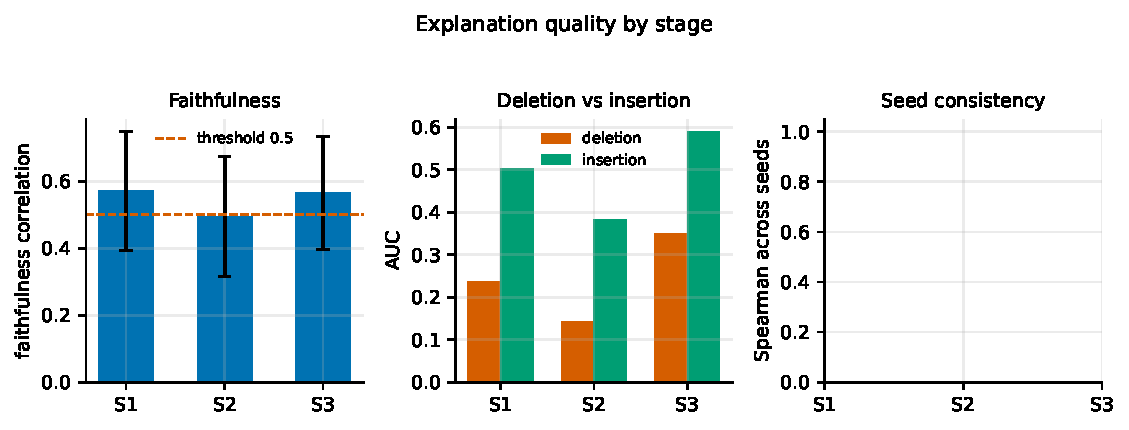
\includegraphics[width=\linewidth]{fig4_explanation_quality.pdf}
\caption{Explanation quality by stage: faithfulness correlation against its
pre-registered threshold; deletion versus insertion AUC; and Spearman agreement of
the importance ordering across the five frozen seeds.}
\label{fig:quality}
\end{figure}

\textbf{Seed consistency passes decisively} at every stage, with a worst-pair
correlation of 0.886 against a threshold of 0.6. This is what licenses
Figure~\ref{fig:migration}: the migration trajectory survives reseeding.

\textbf{Deletion AUC is roughly half insertion AUC at every stage}, and removing top
positively-attributed features degrades the prediction monotonically. The
explanations point at features the model genuinely uses.

\textbf{Faithfulness is stage-dependent, and S2 misses the pre-registered
threshold} (0.494 against 0.5). We report this as a failure against the stated bar
rather than rounding it up.

\subsection{Cross-paradigm agreement (H4)}
\label{sec:h4}

The GRU is competitive with the tree models---test PR-AUC 0.124 against 0.131 at S1
and 0.565 against 0.568 at S3---so any disagreement below is not attributable to one
incompetent arm.

At the level of \textbf{aggregate feature rankings}, Spearman correlations between
TimeSHAP and TreeSHAP are $+0.200$ (S1), $+0.500$ (S2) and $+0.600$ (S3), against a
pre-registered threshold of 0.6. \textbf{H4 is not supported.} However, this test is
severely underpowered: the two paradigms share only four or five mappable concepts,
and with four items Spearman can take only a handful of discrete values. The
pre-registration did not anticipate how few concepts the schemas would share.

We therefore also computed agreement \textbf{per instance}: for each concept, the
tree and sequence attributions were correlated across 350+ shared sessions, over
five seeds (Table~\ref{tab:h4}).

\begin{table}[t]
\centering
\caption{Cross-paradigm agreement, aggregate versus per instance. Per-instance
values are means over five seeds; ``sign-stable'' counts concepts whose correlation
keeps its sign across all five.}
\label{tab:h4}
\small
\begin{tabular}{@{}lS[table-format=+1.3]S[table-format=+1.3]c@{}}
\toprule
\textbf{Stage} & {\textbf{Aggregate $\rho$ (5 concepts)}} &
{\textbf{Per-instance mean $\rho$}} & \textbf{Sign-stable} \\
\midrule
S1 & +0.200 & +0.179 & 1 of 4 \\
S2 & +0.500 & -0.018 & 0 of 5 \\
S3 & +0.600 & +0.046 & 2 of 5 \\
\bottomrule
\end{tabular}
\end{table}

Per-instance agreement is \textbf{indistinguishable from zero at every stage}, and
only 3 of 14 (stage, concept) pairs hold a consistent sign across seeds.
\textbf{Aggregate convergent validity does not imply agreement about individual
cases.} The same models produce aggregate correlations up to $+0.600$ and
per-instance agreement of approximately zero.

We note explicitly that a single-seed version of this analysis produced an apparent
$-0.151$ at S2 that did \emph{not} survive reseeding (Appendix~A). With seed
standard deviations of 0.2--0.4 on these correlations, sign stability rather than
the mean is the reportable quantity.

\subsection{Sensitivity analyses}
\label{sec:sensitivity}

\paragraph{Sessionisation gap.}
Halving or doubling the 30-minute inactivity threshold changes the session count by
$\pm3\%$, stage reach by under one percentage point and stage prevalence by well
under half a point---all far smaller than the between-stage differences on which
the paper's claims rest (Table~\ref{tab:gap}).

\begin{table}[t]
\centering
\caption{Sessionisation gap sensitivity. Reach and prevalence are reported per
stage as reach\,/\,prevalence.}
\label{tab:gap}
\small
\begin{tabular}{@{}lS[table-format=7.0]ccc@{}}
\toprule
\textbf{Gap} & {\textbf{Sessions}} & \textbf{S1} & \textbf{S2} & \textbf{S3} \\
\midrule
15 min & 5544851 & 0.978 / 0.0864 & 0.471 / 0.0652 & 0.092 / 0.5160 \\
30 min & 5366181 & 0.979 / 0.0885 & 0.480 / 0.0683 & 0.093 / 0.5210 \\
60 min & 5219040 & 0.979 / 0.0897 & 0.487 / 0.0705 & 0.093 / 0.5248 \\
\bottomrule
\end{tabular}
\end{table}

\paragraph{Sample size.}
Doubling the subsample to 400,000 users changes PR-AUC by $+0.003$ to $+0.009$ and
leaves every conclusion intact: lift still falls monotonically (1.84, 1.49, 1.10)
and ROC-AUC with it (0.648, 0.634, 0.570). Because the sample is nested at a fixed
seed, the 400,000-user set is a strict superset of the 200,000-user set, so these
differences are attributable to the added users rather than to a different draw.

\paragraph{Calibration set.}
Fitting the calibrator on the validation month rather than on a slice of the
training period raises Expected Calibration Error from 0.025 to 0.118
(Figure~\ref{fig:reliability}).

\begin{figure}[t]
\centering
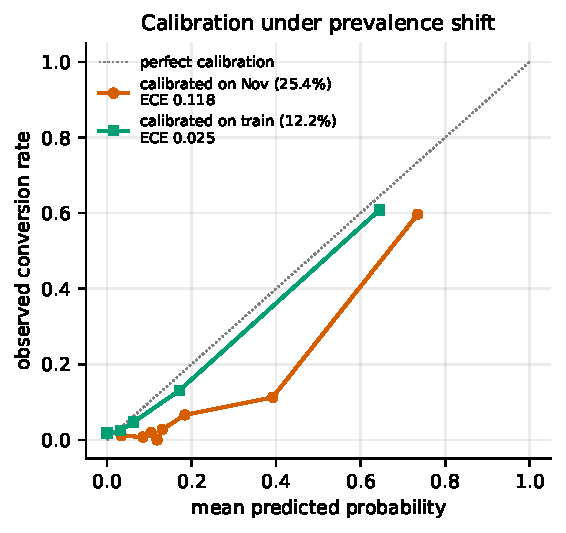
\includegraphics[width=0.72\linewidth]{fig5_reliability.pdf}
\caption{Reliability under prior-probability shift. Calibrating on November
(25.4\% prevalence) and evaluating on December (12.5\%) over-predicts in every
bin; calibrating on a training-period slice (12.2\%) restores calibration.}
\label{fig:reliability}
\end{figure}

%==============================================================================
\section{Discussion}
%==============================================================================

\subsection{Why predictability declines as intent forms}

The clearest result of the study contradicts its own pre-registered hypothesis:
normalised predictive performance \emph{falls} across the funnel. Because this is a
negative result against a directional hypothesis, it deserves a substantive
mechanism rather than a technical dismissal, and the design permits us to rule out
the obvious artefacts.

Three candidate explanations can be excluded. \emph{Prevalence} cannot account for
it: ROC-AUC is invariant to class balance and declines in step with the lift
(Table~\ref{tab:stagemodels}). \emph{Feature availability} cannot account for it
either, and in fact runs the other way---S1 achieves the highest lift with the
\emph{fewest} features (19 against 23), because cart-derived features are excluded
by construction (Section~\ref{sec:stages}). \emph{Sampling noise} is implausible at
seed standard deviations one to two orders of magnitude below the between-stage
gaps, and the ordering is unchanged when the sample is doubled
(Section~\ref{sec:sensitivity}).

What remains is a substantive account. Conditioning on cart possession is a strong
behavioural filter: it removes the browsers, leaving a population that converts
52\% of the time. Within that population the residual variance in the outcome is
governed by factors the clickstream does not observe---checkout friction, payment
failure, unexpected delivery cost, external interruption---rather than by browsing
behaviour, which has become homogeneous. In information terms, the prefix carries
progressively less of the information required to separate the classes as the
population is refined, even as the base rate rises. Early in the journey, by
contrast, browsing behaviour is the \emph{only} thing that distinguishes visitors,
and it discriminates comparatively well.

This reading generates a testable implication we could not evaluate here: adding
off-stream covariates (payment method, delivery quote, checkout latency) should
recover predictability at S3 while leaving S1 largely unchanged. If it does not,
the mechanism is wrong and the decline reflects something about the model class
rather than the information available.

\subsection{Attribution migration and the staged view of the journey}

The behavioural arm of H2 is supported, and this is consistent with a staged view of
the consumer journey in which context gives way to demonstrated behaviour as intent
forms \citep{lemon2016understanding,moe2003buying}.

The result H2 did not predict is more interesting. Navigation entropy peaks at
consideration and collapses at intent (Table~\ref{tab:migration}). Journey theory
tends to treat exploration as decaying steadily as intent forms; these data suggest
instead that exploratory breadth is a \emph{stage-specific diagnostic}---informative
exactly where the visitor is choosing among alternatives, uninformative once the
choice is made. This is consistent with \citeauthor{moe2003buying}'s
(\citeyear{moe2003buying}) typology of visit purpose, in which deliberation is a
distinct mode rather than a point on a monotone intent scale: entropy is
high-information precisely when the visitor is in that mode.

A monotone framing of the funnel cannot express this pattern, which is the
substantive argument for stage conditioning as a modelling commitment rather than a
reporting convenience. It also bears on the interpretation of static SHAP summaries
in this literature: a driver whose importance is concentrated in one phase will
appear middling in a whole-session analysis, and will be discarded during feature
selection for the wrong reason.

\subsection{Implications for practice}

Two implications follow, and they point in the same direction.

First, \textbf{intervention should be concentrated early}. If late-stage prediction
is close to chance relative to its base rate (lift 1.09 at S3), then models cannot
usefully discriminate among cart-holders, and effort spent scoring them is largely
wasted. This runs against the concentration of cart-abandonment tooling in the
industry. The prescription is not that cart abandonment is unimportant---it is that
\emph{targeting} within the cart-holding population is poorly supported by
behavioural data, so undifferentiated treatment may be the rational policy there
while differentiated treatment is justified earlier.

Second, \textbf{the actionable signal is stage-specific}. Navigation entropy is the
clearest case. A whole-session analysis reports a share of 0.111 and would rank it a
minor driver, where it in fact reaches 0.224 at consideration---a value the static
figure never takes at any stage (Table~\ref{tab:static}). An intervention targeting
wandering behaviour has purchase during consideration and close to none at cart.

\begin{table}[t]
\centering
\caption{What a static whole-session attribution would flatten. ``Static share'' is
the stage-averaged attribution a pooled analysis reports; ``range'' is how far the
driver actually travels across stages.}
\label{tab:static}
\small
\begin{tabular}{@{}lS[table-format=1.3]S[table-format=1.3]S[table-format=1.3]l@{}}
\toprule
\textbf{Driver} & {\textbf{Static share}} & {\textbf{Range}} &
{\textbf{Peak}} & \textbf{Peak stage} \\
\midrule
Engagement and tempo    & 0.292 & 0.199 & 0.368 & S2 \\
Price                   & 0.352 & 0.198 & 0.437 & S1 \\
Navigation and category & 0.111 & 0.189 & 0.224 & S2 \\
Products viewed         & 0.094 & 0.159 & 0.192 & S1 \\
\bottomrule
\end{tabular}
\end{table}

We note the necessary precondition: acting on predicted probabilities requires them
to be calibrated, which the next subsection shows is easy to get wrong.

\subsection{Methodological implications}

Three findings hold independently of the framework and may transfer more readily
than the framework itself.

\paragraph{A canonical benchmark drifts, and is usually split randomly.}
Conversion prevalence in Dataset~A rises almost monotonically from 1.6\% in February
to 25.4\% in November before halving to 12.5\% in December---a fifteen-fold range.
Random splitting mixes these months and conceals the drift. Our month-ordered
results are consequently lower than those commonly reported on this benchmark, and
we regard that as a correction rather than an underperformance. The general point is
that a benchmark's temporal structure should be inspected before a splitting
protocol is chosen, even when the benchmark is nominally cross-sectional.

\paragraph{Prior-probability shift destroys calibration, and the remedy is the
calibration set, not a post-hoc correction.}
Fitting the calibrator on November (25.4\% prevalence) and applying it to December
(12.5\%) produced a mean predicted probability of 0.2421 against an observed rate of
0.1251---a ratio of 1.935, almost exactly the prevalence ratio of 2.03---with
over-prediction in every reliability bin (Figure~\ref{fig:reliability}).
Discrimination was unaffected, since ranking is invariant to monotone
miscalibration. Notably, applying the EM prior-shift correction of
\citet{saerens2002adjusting} \emph{on top of} a correctly drawn calibration set made
calibration \textbf{worse} for every model, since it estimated a prior of 0.1447
against a true 0.1251 and over-corrected a shift that was no longer present. The
instinct is to reach for the correction; the answer is to fix the split.

\paragraph{Aggregate convergent validity does not imply per-instance agreement.}
Two attribution paradigms produced aggregate rank correlations up to $+0.600$ on the
same models while agreeing approximately not at all about which individual journeys
each driver mattered for (Section~\ref{sec:h4}). The two quantities answer different
questions, and only the second is relevant to a practitioner reasoning about a
specific case. Any study claiming convergent validity between explanation methods
should therefore report per-instance agreement; aggregate agreement over a handful
of concepts is both easier to achieve and weaker evidence than it appears.

\subsection{When should an explanation be trusted?}

Three independent measurements converge on the same stage. Consideration (S2) has
the weakest predictive lift (1.41), the only faithfulness score below its
pre-registered threshold (0.494), and the lowest aggregate cross-paradigm agreement.
The common factor is signal: S2 is where the model has least to work with, and where
its explanations are correspondingly least trustworthy.

If this relationship generalises, it has a practical consequence for XAI reporting.
Explanation quality is normally reported per model, as a single faithfulness or
stability number. Our results suggest it should be reported \emph{per stratum}---per
stage here, but plausibly per segment, per period or per cohort elsewhere---because
a model-level average conceals exactly the strata where the explanation should not be
acted upon. This is the most portable claim in the paper, and the one we would most
like to see tested on other data.

We are careful not to overstate it. Three measurements on one dataset establish a
pattern, not a law; a fourth signal that appeared to support it was withdrawn after
reseeding (Appendix~A), which is itself a caution against reading too much into
convergence among small numbers of measurements.

\subsection{Limitations and threats to validity}

\paragraph{Absent variables.} Search-query text is unavailable in both datasets and
scroll depth is proxied by dwell time (Table~\ref{tab:availability}). Device and
traffic source are absent from Dataset~B, so H2's context arm is untestable there.

\paragraph{Dataset~A is non-causal by construction.} Its features are whole-session
aggregates and \texttt{PageValues} is measured post-transaction. It functions as a
benchmark and as the static comparator, not as a causal model.

\paragraph{Stage models are conditional on reaching the stage.} The improvement
curve is a conditional claim, and Table~\ref{tab:stages} reports the reach rates and
prevalences needed to read it as such.

\paragraph{The intent stage is underpowered.} With 2,973 test sessions, no S3
ablation contrast is decidable. This is a sample-size limitation and argues for a
wider observation window.

\paragraph{The temporal split discards data.} Keeping visitors whole \emph{and}
respecting time order costs 51,256 of 200,000 users as boundary-straddlers,
retaining 222,268 of 485,459 sessions. A window longer than one month would reduce
this fraction substantially.

\paragraph{The recurrent arm is small.} The GRU is trained briefly on a subsample,
and its attributions carry seed standard deviations of 0.2--0.4. Conclusions from it
are correspondingly weak, and one single-seed conclusion had to be withdrawn.

\paragraph{External validity.} One retailer, one market, one month. The framework is
portable; these specific attribution trajectories are not claimed to be.

\subsection{Future work}

Priorities, in order: a multi-month observation window, which addresses both the S3
power limitation and the temporal-split attrition; the off-stream covariate test
proposed above, which would falsify or support the mechanism offered for the
declining curve; prevalence-corrected calibration for deployment under seasonal
drift; a larger sequence model to test whether the per-instance disagreement is a
property of the paradigms or of an under-trained GRU; and live A/B validation of the
early-funnel intervention implied above.

%==============================================================================
\section{Conclusion}
%==============================================================================

We proposed a funnel-stage SHAP framework that conditions Shapley attributions on
journey stage, computes them strictly on the event prefix available at each stage,
and validates them for faithfulness, stability and reproducibility. Applied to 42.4
million clickstream events and a canonical session-level benchmark, it produced
three results that a whole-session analysis could not have produced.

Normalised predictive performance falls rather than rises across the funnel, so
conversion becomes harder to predict as intent forms, and the useful intervention
window is earlier than industry practice assumes. Attribution is strongly
non-monotone, with navigation entropy mattering at consideration and nowhere
else---a pattern any single whole-session attribution averages away. And convergent
validity between explanation paradigms, which holds at the level of aggregate
rankings, disappears at the level of individual journeys.

Three of the four pre-registered hypotheses were not supported. We report them as
such. The practical recommendation for researchers applying SHAP to consumer-journey
data is narrower than the framework itself: \textbf{validate explanations per stage
rather than per model}, because explanation quality tracks predictive signal, and a
stage-averaged quality metric conceals exactly the stages where the explanation
should not be trusted.

%==============================================================================
\section*{Declarations}
%==============================================================================

\paragraph{CRediT author statement.} Ayoub Agnaou: Conceptualization, Methodology,
Software, Formal analysis, Data curation, Writing -- original draft, Writing --
review \& editing, Visualization.

\paragraph{Declaration of competing interest.} [To complete.]

\paragraph{Declaration of generative AI in the writing process.}
\textcolor{red}{[To complete, and to complete accurately. Generative AI was used
substantially in implementing the analysis code and in drafting this manuscript.
State this in the form the target journal specifies; do not understate it.]}

\paragraph{Data availability.} Dataset~A is publicly available from the UCI Machine
Learning Repository under CC~BY~4.0 \citep{sakar2019real}. Dataset~B is published
openly by the REES46 Marketing Platform. \textcolor{red}{No formal licence text is
published for Dataset~B}; the files are distributed without a click-through licence
and are widely used in published work, but a specific grant of rights for research
publication could not be located. This position is stated here rather than a licence
asserted. [Obtain written confirmation from REES46 before submission and replace
this paragraph.]

\paragraph{Code availability.} The complete analysis pipeline, frozen data splits,
seed list, environment lockfile and amendment log are available at
[repository URL].

\paragraph{Ethics.} Behavioural data only; no personally identifying information.
Identifiers were pre-hashed by the publisher and no re-identification was attempted.
Explanations are reported at cohort level.

\paragraph{Funding.} [To complete.]

%==============================================================================
\appendix
\section{Pre-registered protocol and amendment log}
%==============================================================================

The pre-registered protocol (v1.0) and the complete dated amendment log (23
entries) accompany this manuscript. Amendments record every deviation from the
frozen protocol with its date, rationale and affected sections, including three
cut-point redefinitions made on the basis of measurement
(Section~\ref{sec:stages}), one reversal of a reported hypothesis verdict after
proper confidence intervals replaced an invalid comparison of means to seed
standard deviations, and one withdrawal of a single-seed result that did not
survive reseeding (Section~\ref{sec:h4}).

%==============================================================================

\bibliographystyle{elsarticle-harv}   % FALLBACK: use \bibliographystyle{apalike}
\bibliography{references}

\end{document}
